\chapter{Evaluation}
\label{chapter:evaluation}

In this chapter we present the evaluation of \cottontail{} \cite{Gasser:2020Cottontail}, which implements the previously described concepts and has become an integral part of the \vitrivr{} \cite{Rossetto:2016vitrivr,Gasser:2019Towards,Gasser:2019Multimodal} stack. For this quantiative evaluation, we focus on three aspects:

\begin{description}
    \item[Interactive Multimedia Retrieval Workloads] These benchmarks focus on interactive video retrieval workloads on million-scale datasets, for which \cottontail{} was primarily designed. We demonstrate \cottontail{}'s versatility and discuss and compare different execution plans (index, multi-threading, \acrshort{simd}). For this evaluation, we use the Vimeo Creative Commons Collection 1 \& 2 (V3C) \cite{Berns:2019V3C1,Rossetto:2021Insights}, which currently serves as the reference dataset for both \acrshort{vbs} and TRECVID AVS. The dataset consists of 17235 videos, which amounts to \SI{2300}{\hour} of content. We use a series of features derived by \vitrivr{}'s feature extraction engine Cineast as listed in \Cref{table:datasets}.
    \item[Large-Scale Similarity Search] In these tests, we examine how \cottontail{} scales out to billion-scale datasets as employed in challenges such as the (Big-) ANN-Benchmark \cite{Aumueller:2017ANN,Simhadri:2022Results}. While not the primary focus of \cottontail{}'s design, this is still an interesting task to obtain a baseline for future efforts. We use this opportunity to compare \cottontail{} to Milvus (see \Cref{section:milvus}) in a series of large-scale \acrshort{nns} queries. All queries are run against shards of the Yandex Deep1B dataset \cite{Babenko:2016Efficient}, which is a collection of descriptors derived from a GoogLeNet \cite{Szegedy:2015Going} neural network.
    \item[Adaptive Index Management] This test examines \cottontail{} ability to cope with changes to datasets and associated index structures that take place concurrently. We demonstrate the deterioration of indexing quality and the automated mechanisms that maintains up-to-date indexes.
\end{description}

\section{Evaluation Setup}

The entire evaluation is centered around database queries that are sent to the system under testing. We generate measurements from these queries and the results they return. Typically, we average the obtained values over $10$ repetitions in order to compensate for anomalies and we execute a single warm-up query to give the system's the ability to initialise necessary caches. 

Rather than working with randomly generated data, we decided to use existing data corpora that reflect the structure of features as generated by different, real-world models. Those data sets are listed in \Cref{table:datasets} and we will refer to the collections and entities by their name throughout this chapter. For the the Yandex Deep1B \cite{Babenko:2016Efficient} dataset we have prepared different shards that contain the first 5 million, 10 million, 100 million and all 1 billion vectors. All data is imported as a dedicated entity (\cottontail{}) or collection (Milvus) respectively, prior to executing the actual workloads. Index structures are also prepared beforehand if not stated otherwise. Every entity exhibits the columns \texttt{id} and \texttt{feature}. The \texttt{id} column serves as a primary key and is either a \texttt{string} (all V3C-based datasets) or a \texttt{long} value (all Deep1B-based datasets). The Deep1B shards also exhibit an additional \texttt{category} column, which holds a randomly assigned \texttt{int} value that is used for Boolean filtering. The Deep1B datasets also come with query vectors and groundtruth data, which we use accordingly.

\begin{table}
    \begin{tabular}{ | l | c | c | c | p{5cm} |}
        \hline
        \textbf{Entity} & \textbf{Source} & \textbf{d} & \textbf{N} & \textbf{Description} \\
        \hline
        \hline
        features\_averagecolor & V3C1\&2  & 3 & 2512715 & Average colours derived from video segments. \\ 
        \hline
        features\_visualtextcoembedding & V3C1\&2 & 25 & 2506273 & Video to text co-embedding derived from vide segments. See \cite{Spiess:2021Competitive}. \\
        \hline
        features\_hogmf25k512  & V3C1\&2  & 512 & 2500943 & HOG \cite{Bay:2006surf} describtors derived from video segments. \\
        \hline
        features\_inceptionresnetv2 & V3C1\&2  & 1536 & 2508358 & Vector derived from last fully connected layer of a pre-trained InceptionResNetV2 applied on video segments.\\
        \hline
        features\_conceptmasksade20k & V3C1\&2 & 2048 & 2469844 & Image embedding for query by semantic sketch. See \cite{Rossetto:2019Query}. \\
        \hline
        yandex\_deep5M  & Deep1B  & 96 & $5000000$ & See \cite{Babenko:2016Efficient} for more details. \\
        \hline
        yandex\_deep10M  & Deep1B & 96 & $10000000$ & See \cite{Babenko:2016Efficient} for more details. \\
        \hline
        yandex\_deep100M  & Deep1B & 96 & $100000000$ & See \cite{Babenko:2016Efficient} for more details. \\
        \hline
        yandex\_deep1B  & Deep1B & 96 & $1000000000$ & See \cite{Babenko:2016Efficient} for more details. \\
        \hline
        \hline
    \end{tabular}
    \caption{The data collections used for this evaluation. }
    \label{table:datasets}
\end{table}

Both \cottontail{} and Milvus are deployed on the same physical server but they do not run concurrently. This server exhibits two \acrshort{numa} nodes with an Intel Xeon CPU E5-2630 v4 (20 cores@\SI{2.2}{\giga\hertz}) and \SI{192}{\giga\byte} \acrshort{ram} each. Therefore, the machine provides 40 compute cores and a total of \SI{384}{\giga\byte} of \acrshort{ram}. The \acrshort{cpu} supports the AVX2 instruction set extension, which allows for vectorised execution. The data directories from which Milvus and \cottontail{} access their data resides on three \SI{500}{\giga\byte} \acrshort{ssd}'s that have been combined into a single, logical disk using \acrshort{raid}0 (striping). The server runs Ubuntu 20.04 and the OpenJDK Java version 17.0.3. All queries are sent from a separate computer on the same network to minimise the impact on query execution. The evaluation scripts are available online\footnote{See https://github.com/ppanopticon/cottontaildb-evaluation/, Accessed July 2022}.

The binary version of \cottontail{} is started with a minimum and maximum heap size of \SI{64}{\giga\byte} and \SI{256}{\giga\byte} respectively. Furthermore, we have activated \acrshort{simd} support in the JVM in form of Java's new \emph{Vector API} \footnote{See https://openjdk.org/jeps/, JEPs 338, 414 and 417, Accessed July 2022} by loading the corresponding incubator module. In terms of configuration we have setup \cottontail{}'s default cost model in a way that makes it parallelise workloads aggressively whereas, by default, it tries to limit its resource use. The set of configuration parameters including explanation can be found in \Cref{chapter:appendix_results}.

For Milvus, the basic setup is identical to that used for \cottontail{}, i.e., Milvus runs on a single node, despite its ability to scale out to large clusters, in order to keep the setup comparable. We use the Milvus standalone version and we followed the official tutorial for setting it up \footnote{See https://milvus.io/docs/v2.0.x/, Accessed July 2022}. All benchmarks were conducted with the latest version 2.0.2 without further adjustments to the default configuration. In this default state, Milvus is allowed to use all available resources in terms of \acrshort{cpu}, \acrshort{ram} and disk space.

\subsection{Metrics}

We assume that for every query, we receive a list of results $R$ from the respective database. That list contains $K$ items $r_i \in R, i \in \lbrack 1, K  \rbrack $ that match the query. The returned items $r_i$ are ranked either explicitly based on score or distance (for \acrshort{nns}, \acrshort{fns} or range search) or just arbitrarily, i.e., $r_1$ comes at position one, $r_2$ at position two and so forth. The ranking is solely dependent on the database and query. Every item $r_i$ is simply a tuple containing the primary key of the retrieved database entry, which we always use to test for equality.

For every query, we are interested in assessing the efficiency and effectiveness of its execution. Efficiency can be easily gauged in terms of query execution time, which is the elapsed real time in seconds between issuing the query and receiving the results. This metric is simple enough to obtain and reason about and does not require further elaboration. The effectiveness of the query, i.e., the quality of the results it produces, is a bit more complicated and therefore assessed by two separate metrics: Given a result $R$ produced by the database and a known groundtruth $G$, i.e., a list of results that we know to be correct, we obtain both the recall as well as the \acrfull{dcg} \cite{Jarvelin:2002Cumulated} of the result compared to the groundtruth at a given level $k \leq K$. Henceforth, we will use $k$ as subscript to indicate, that a fixed number if items is considered.

The reason for obtaining two metrics for result quality lies in the limitations of the metrics themselves. Recall at a fixed level $k$, for which a definition is provided in \Cref{equation:recall}, is purely set-based and simply checks for the existence of an element from the groundtruth $G_k$ in the result $R_k$, without taking the exact positioning of the items into account.

\begin{equation}
    \label{equation:recall}
    \texttt{REC}_k (R_k, G_k) = \frac{|R_k \cap G_k |}{k}
\end{equation}

If $R_k$ contains items that are not contained in the groundtruth (false positives) or $G_k$ contains documents that are missing in $R_k$ (false negative), this directly results in a drop in $\texttt{REC}_k$. Therefore, if all of the items $r_i \in R_k$ were to be contained in $G_k$, i.e., $R_k \cap G_k = G_k$, the recall would become $1.0$ and a result could be considered a perfect match. In contrast, if none of the items in $r_i \in R_k$ were contained in $G_k$, i.e., $R_k \cap G_k = \emptyset$ then recall drops to $0.0$. However, recall does not provide us with any information about the ranking of the individual items. In an extreme case, two lists containing the same items but in a reversed order would produce the same recall value of $1.0$. Often, though, we find that items with a low rank are more important than items with a very high rank. This is true both when considering a human user browsing a list from top to bottom, typically paying attention only to the top entries, or a use-case in which we are only interested in the top item(s) (see, for example, \Cref{section:application_mrf}). Nevertheless, and despite these limitations, the recall metric and variants thereof are very popular in \acrshort{anns} evaluations \cite{Aumueller:2017ANN,Simhadri:2022Results}. 

To compensate for the absence of information about the ranking quality, we turn to a variant of the \acrshort{dcg} at a given level $k$, which in its original form was proposed by \cite{Jarvelin:2002Cumulated}. Our adapted version is specified in \Cref{equation:dcg}. It builds the sum over all items $r_i \in R_k$. The numerator of the expression specifies the assigned relevance of an item based on its position in the groundtruth $G_k$, which is expressed by the function $\text{rel} (r_i)$. If $r_i$ has rank $1$ in $G_k$, it is considered most relevant and thus receives the relevance $k$. If $r_i$ has rank $k$ in $G_k$, it is not considered very releveant and therefore receives the relevance $1$. If $r_i$ is not contained in $G_k$ at all (false positive), then $\text{rank} (g_i)$ returns the lowest possible gain $0$. The denominator is the logarithm of the actual rank of $r_i \in R_k$. 

\begin{eqnarray}
\label{equation:dcg}
\mathtt{DCG}_k (R_k, G_k)= \sum_{i = 1}^{k} \frac{\text{rel}(r_i) + 1}{\log_2(i + 1)} \\
\text{rel} (r_i) = 
    \begin{cases}
        k - \text{rank}_{G_k}(r_i), &  \text{if } r_i \in G_k \\
        0,                          &  \text{if } r_i \notin G_k
    \end{cases}
\end{eqnarray}

The reasoning behind using this \acrshort{dcg} variant is that items with a low rank in $G_k$ are more important than items with a very high rank. The numerator accounts for this by assigning high relevance to items that appear early on, which quantifies the gain of inspecting such an item. That gain is discounted by an item's actual rank in $R_k$, i.e., the further down in the list an item appears the larger the discount. Obviously, if an item in the result $R_k$ does not appear in the groundtruth (false positive), then there is no gain at all. What is not directly captured by the \acrshort{dcg}, however, are entries that appear in $G_k$ but that are missing in $R_k$ (false negatives). However, this is again covered by the recall. To make the \acrshort{dcg} values comparable across queries (potentiall with different values of $k$), we normalise it by the ideal $\mathtt{iDCG}_K$ to obtain the normalised $\mathtt{nDCG}_K$ as indicated by \Cref{equation:ndcg}. The $\mathtt{iDCG}_K$ simply quantifies the maximum perfect ranking given groundtruth $G_K$. Therefore, the normalised $\mathtt{nDCG}_K$ always assumes values between $0.0$ and $1.0$. All the metrics described here are also illustrated in \Cref{example:result_and_metrics}.

\begin{align}
    \label{equation:ndcg}
    \mathtt{nDCG}_k(R_, G_k) &= \frac{\mathtt{DCG}_k(R_K, G_K)}{\mathtt{iIDCG}_K(G_K)} \\
    \mathtt{iIDCG}_k(G_k) &= \sum_{i = 0}^{K} \frac{k + 1 - i}{\log_2(i + 1)}
\end{align}

\begin{example}[label=example:result_and_metrics]{Result $R$, Groundtruth $G$ and obtained metrics.}{}
    We consider the following result $R$ and the associated groundtruth $GT$ ($k = 7$), which contain the same items but in exact reverse order.

    \begin{center}
        \begin{tabular}{ l || l | l || l | l | l | l |}
            \textbf{Rank} & \textbf{GT} & $ k + 1 - i$ & \textbf{R} & $R_k \cap G_k$ &  $\text{rel}(r_i)$ & $\log_2(i + 1)$ \\ 
            \hline
            \hline
            $1$ & 87  & 7 & 597  & \cmark & 2 & 2.58 \\
            \hline
            $2$ & 123  & 6 & 331 & \cmark &  3 & 2.32 \\
            \hline
            $3$ & 542 & 5 & 3213 & \cmark & 4 & 2 \\
            \hline
            $4$ & 3213 & 4 & 542 & \cmark &  5 & 1.58 \\
            \hline
            $5$ & 313 & 3 & 123 & \cmark &  6 & 1 \\
            \hline
            $6$ & 597 & 2 & 87 & \cmark &  7 & 1 \\
            \hline
            $7$ & 757 & 1 & 888 & \xmark & 0 & 1 \\
            \hline
        \end{tabular}
    \end{center}


    The values for $\mathtt{REC}_7$, $\mathtt{DCG}_7$, $\mathtt{IDCG}_7$ and $\mathtt{NDCG}_7$ according to Equations \ref{equation:recall}, \ref{equation:dcg} and \ref{equation:ndcg} are given as follows.

    \begin{align*}
        \label{equation:dcg_example}
        \mathtt{REC}_7 &= \frac{6}{7} = 0.86 \\
        \mathtt{DCG}_7 &= \frac{2}{1} + \frac{3}{1.58} + \frac{4}{2} + \frac{5}{2.32} + \frac{6}{2.58} + \frac{7}{2.81} + \frac{0}{3} = 12.87 \\
        \mathtt{IDCG}_7 &= \frac{7}{1} + \frac{6}{1.58} + \frac{5}{2} + \frac{4}{2.32} + \frac{3}{2.58} + \frac{2}{2.81} + \frac{1}{3} = 17.23 \\
        \mathtt{NDCG}_7 &= \frac{12.87}{17.23} = 0.75
    \end{align*}

\end{example}


\section{Execution of Multimedia Analytics Workloads}

This series of measurements is about demonstrating \cottontail{}'s versatility to execute different types of multimedia retrieval workloads. For this, we have prepared a little test protocol that we execute to demonstrate the versatility of the proposed, relational algebra extensions.  We start by obtaining a random vector from the test collection. We then go on to obtain the minimum, maximum and mean distance of all vector from that vector. We then perform a \acrshort{fns} query and check if the distance of the first entry equals the maximum distance. This is basically a sanity check. The executed queries are expressed as Pseudo-SQL in \Cref{listing:analytics_queries}.

\begin{lstlisting}[language=SQL, caption={Pseudo-SQL of the queries executed for the analytics workload evaluation.}, label=listing:analytics_queries, numbers=none]
    /* Select a random vector from collection --> this is the query vector. */
    select feature from <collection> skip <random> limit 1
    
    /* Select minimum, mean and maximum distance from the query vector. */
    select min(euclidean(feature, <query>)) from <collection> 
    select mean(euclidean(feature, <query>)) from <collection> 
    select max(euclidean(feature, <query>)) from <collection> 

    /* Perform a range search. */
    select id, euclidean(feature, <query>) as dst from <collection> where dst = ((<max> - <mean>) / 2) order by dst limit 1000

    /* Perform a farthest neighbour search query. */
    select id, euclidean(feature, <query>) as dst from <collection> order by dst desc limit 1000

    /* Perform sub-select with nested nearest neighbour search. */
    select * from multimedia_segment where segmentid IN (select id from <collection> order by euclidean(feature, <query>) asc limit 1000)
\end{lstlisting}

We run all the queries against the V3C-based collections listed in \Cref{table:datasets}: The dimensionality of the vectors ranges between $3$ and $2048$ and we fix the value of $k = 1000$ for all queries involing a $s,k$-selection. For the benchmark, we prepared the following indexes on the respective entities in \cottontail{}: The \acrshort{pq} index variant for exhaustive search ($2048$ centroids) and a \acrshort{vaf} index ($25$ marks per vector component). In addition to the obtained metrics we also let \cottontail{} report the execution plan it selected for a given query using its \emph{explain query} endpoint. These execution plans are illustrated for the purpose of discussion.

\subsection{Influence of Index Structures}

\subsection{Influence of Vectorisation}

\subsection{Influence of Planner Rules}

For these measurements, we have selectively removed planner rules from \cottontail's query planner to observe the impact it has on the outcome.


\section{Large-Scale Similarity Search}
This series of measurements is a direct comparison between Milvus and \cottontail{} and is about mere performance. We execute all queries on prepared shards of the Deep1B \cite{Babenko:2016Efficient} dataset ($d=96$) with $k=1000$ using different execution strategies and compare the obtained metrics. The shards contain 5 million, 10 million, 100 million and 1 billion $96$-dimensional \texttt{float} vectors and are stored in dedicated collections (Milvus) or entities (\cottontail). The Psudo-\acrshort{sql} of the three types of queries is listed in \Cref{listing:big_nns_query}:
\begin{enumerate*}[label=(\roman*)]
    \item A simple \acrshort{nns} query that only returns the primary key and the distance,
    \item a \acrshort{nns} query that additionaly returns the query vector,
    \item a \acrshort{nns} query with a Boolean filter (hybrid query in Milvus terminology).
\end{enumerate*}

\begin{lstlisting}[language=SQL, caption={Pseudo-SQL of the queries executed for this measurement.}, label=listing:big_nns_query, numbers=none]
    /* Simple NNS without feature vectors. */
    select id, euclidean(feature, <query>) as dst from <collection> order by dst limit 1000
    
    /* NSS that returns feature vectors. */
    select id, feature, euclidean(feature, <query>) as dst from <collection> order by dst limit 1000

    /* Hybrid query without feature vector. */
    select id, euclidean(feature, <query>) as dst from <collection> where category = <category> order by dst limit 1000
\end{lstlisting}

We use the query vectors provided with the Deep1B dataset and establish a groundtruth for each query by executing a brute-force search.

\subsection{\cottontail}
\label{section:evaluation_bignns_cottontail}
For this benchmark, we prepared a selection of indexes on the respective entities in \cottontail{}: Two variants of a \acrshort{pq} index, once organised as a list for exhaustive search ($8$ subspaces, $256$ centroids) and once organised as an inverted list for approximate search ($8$ subspaces, $256$ centroids and $256$ coarse centroids) and a \acrshort{vaf} index. Furthermore, we created a $B^{+}$-Tree index on the column \texttt{categories} which we expect to be beneficial for Boolean search. We again use query hints to nudge \cottontail{} into using certain high-dimensional index structures so as to be able to compare the different query execution strategies. Accross all workloads, we compare the performance of four different types of execution strategies: Sequential scan (no index) and the scan of the \acrshort{vaf} and the (IVF-)\acrshort{pq} indexes.

\begin{landscape}
    \begin{figure}[p]
        \centering
        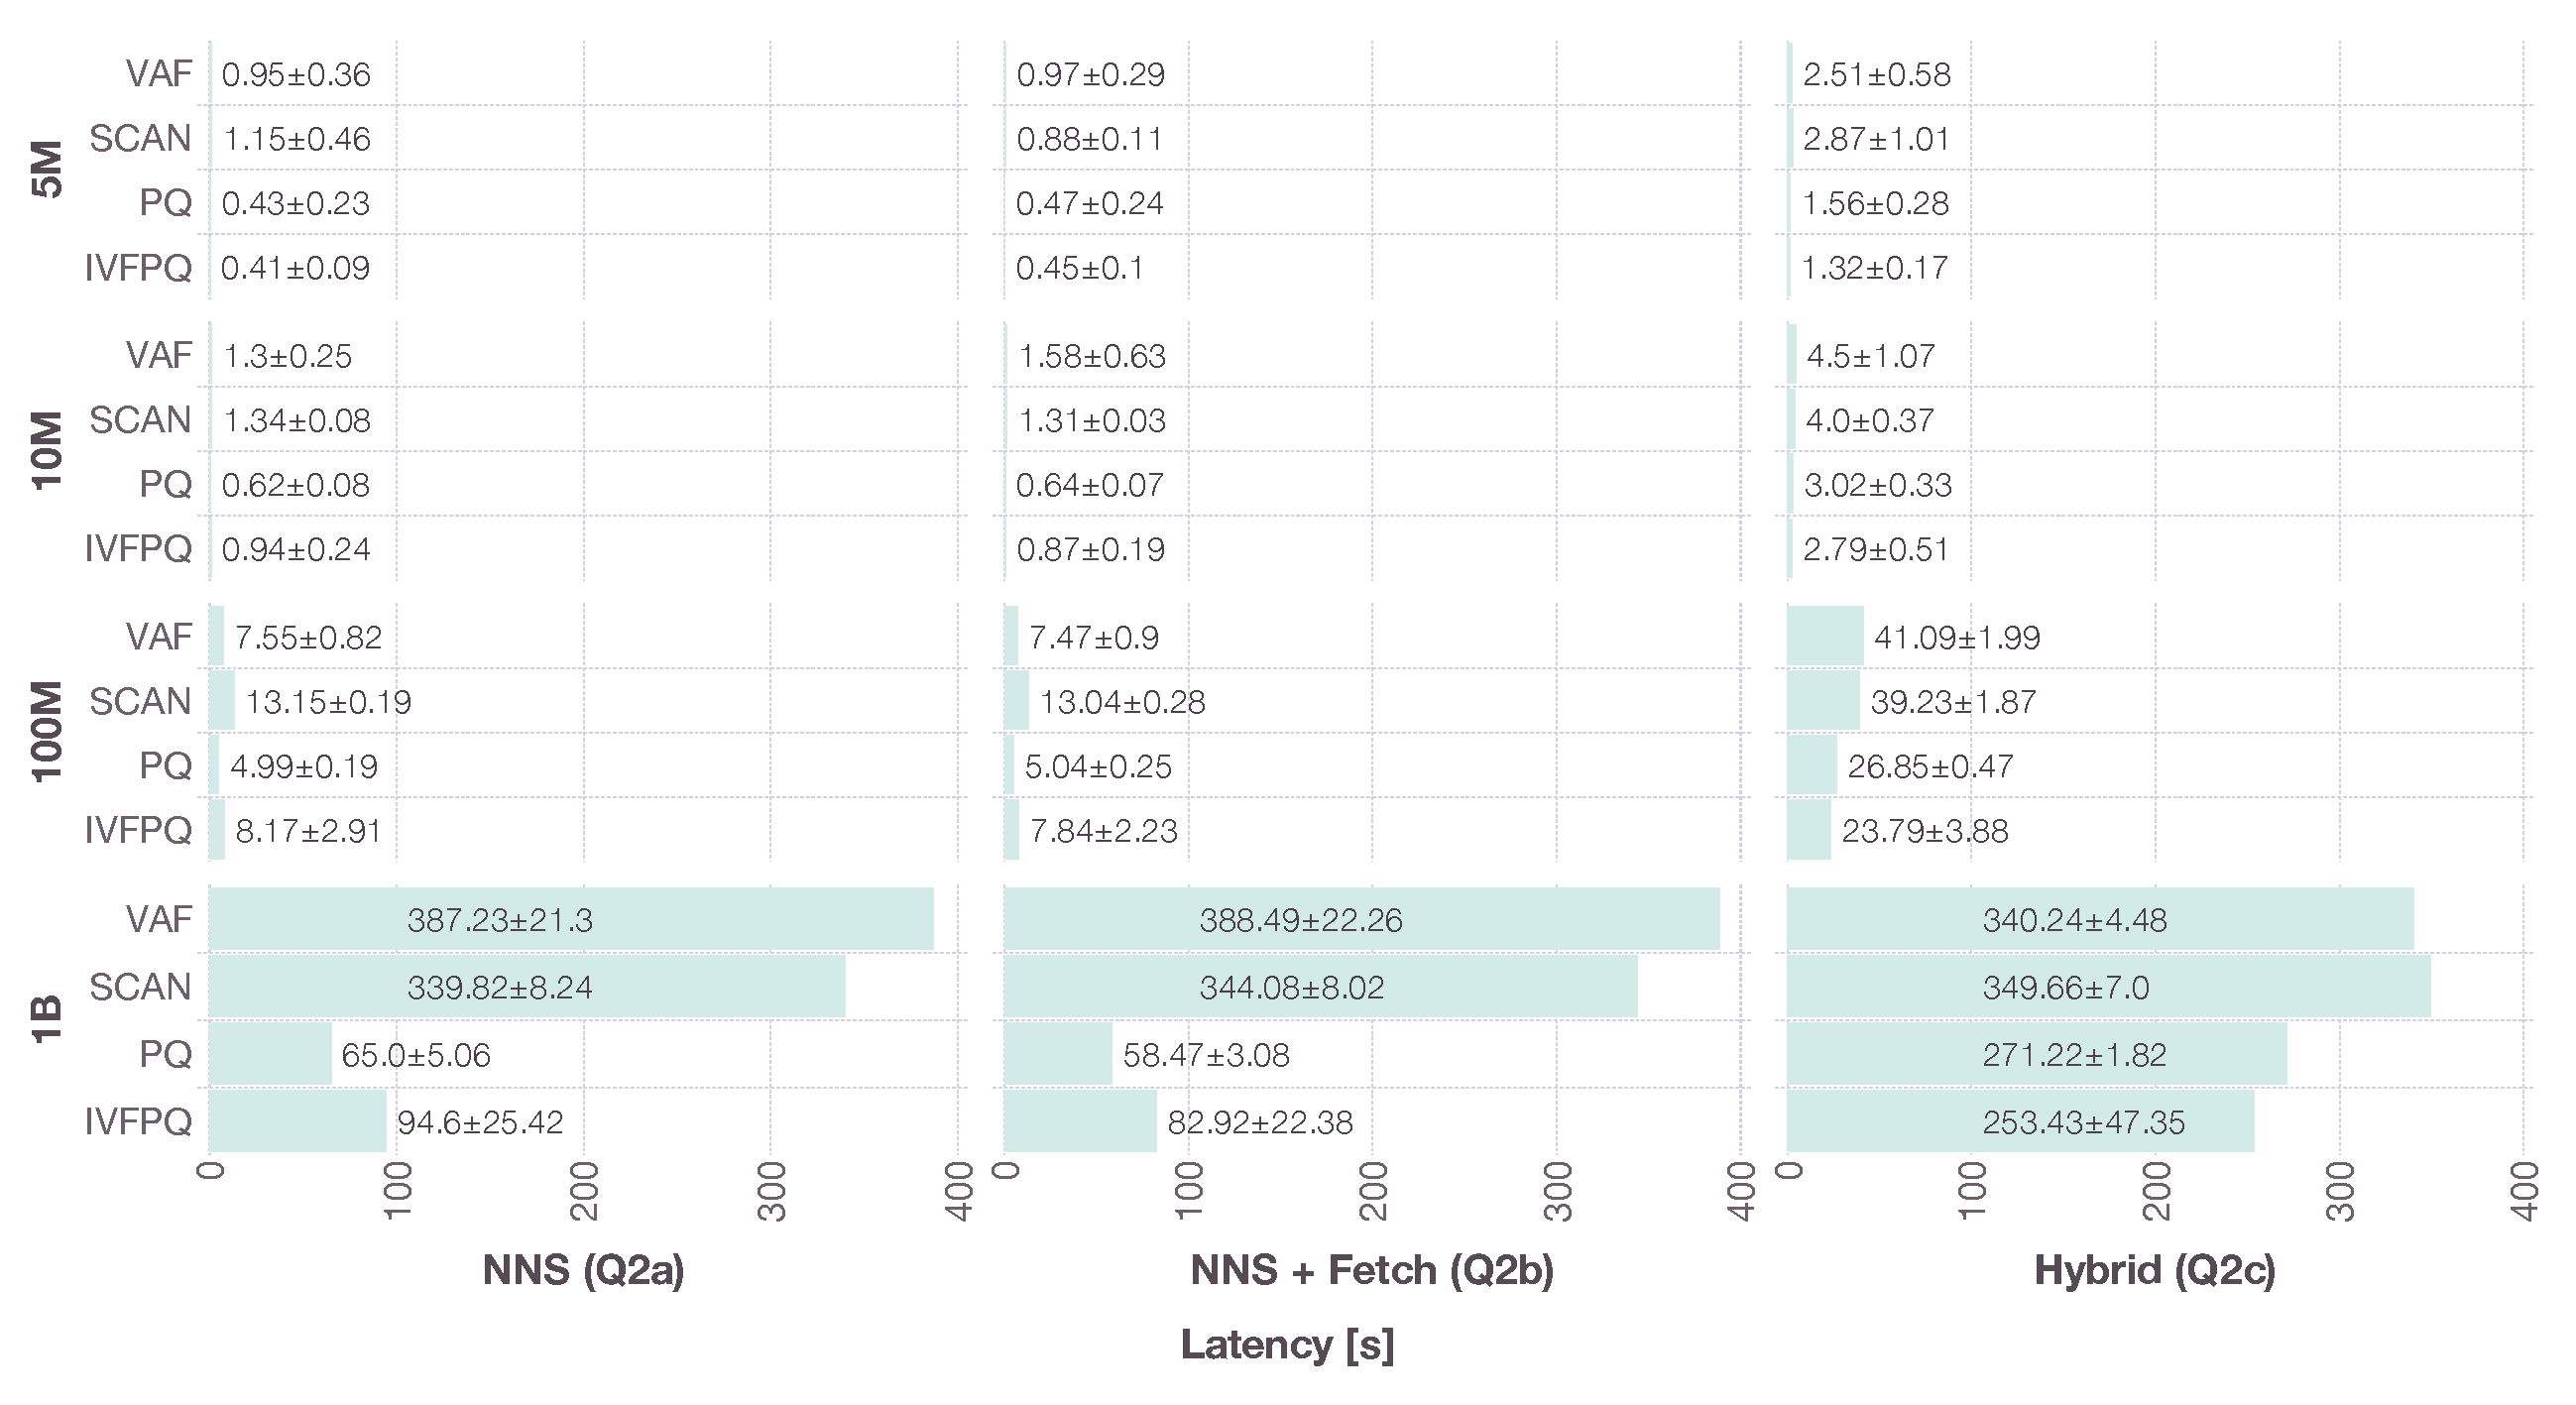
\includegraphics[width=1.55\textwidth]{figures/bignns/cottontail/bignns-cottontail-runtime}
        \caption {\cottontail{}'s latency in seconds for different workloads (x-axis) on different shards of the Deep 1B data set using different access methods (y-axis).}
        \label{figure:cottontail_runtime}
    \end{figure}
\end{landscape}

In our first series of tests we executed the simple \acrshort{nns} workload. The results are depicted in \Cref{figure:cottontail_runtime} (NNS). Brute-force search took between $0.69 \pm 0.12 \, \si{\second}$ (5 million) and $10.45 \pm 0.13 \, \si{\second}$ (100 million). We can observe, that the \acrshort{vaf} index brings only minor advantages for the smaller datasets but reduces execution time by almost \SI{4}{\second} for the larger. This is an artifact of the query execution engine, which uses less than the assigned 32 workes because of the derived \acrshort{cpu} costs. We can also cleary see, that using the (IVF-)\acrshort{pq} index reduces the execution time significantly, but at the cost of impaired quality, which is below $0.5$ for both recall and \acrshort{dcg} (see \Cref{figure:appendix_bignns_cottontail_nns_quality}). However, experience shows that the retrieval quality for these indexes is mainly an issue of tuning the hyperparameters, e.g., the number of coarse and fine centroids used upon index construction. It is also worth noting, that the IVF\acrshort{pq} index does currently not support intra-query parallelism due to \cottontail{}'s partitioning model, i.e., the execution times we see for the IVFPQ index are single-threaded. 

Both \acrshort{pq} and \acrshort{vaf} fail to deliver interactive execution times for very large collections, which can be explained by  the simple fact that these index structures perform an exhaustive search, i.e., they do not limit themselves to a subset of the data. The execution plans are shown in \Cref{figure:cottontail_nns_plan} and is fairly unsurprising: The use of \acrshort{vaf} and \acrshort{pq} constitutes a class 3 resp. class 1 index replacement according to Definitions \ref{definition:dfc_index_class_3} and \ref{definition:dfc_index_class_1}. The fetching of the \texttt{id} columns is pushed down to after the sort and limit operations, since this significantly reduces the amount of IO (only $1000$ fetches instead of several millions).

\begin{figure}[p]
    \centering
    \begin{subfigure}[b]{\textwidth}
        \centering
        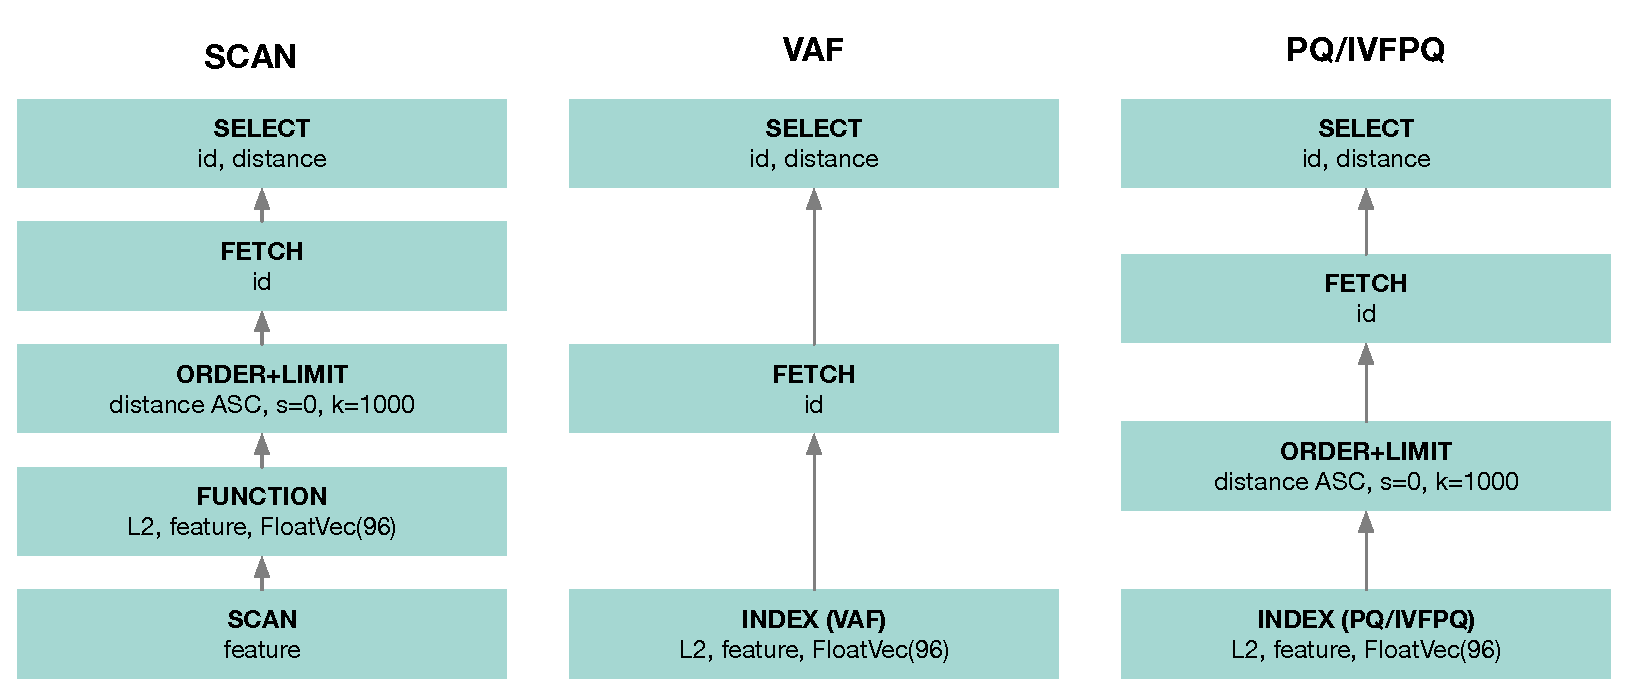
\includegraphics[width=\textwidth]{figures/bignns/cottontail/query-plan-nns}
        \caption{Simple \acrshort{nns}.}
        \label{figure:cottontail_nns_plan}
    \end{subfigure}
    \hfill
    \centering
    \begin{subfigure}[b]{\textwidth}
        \centering
        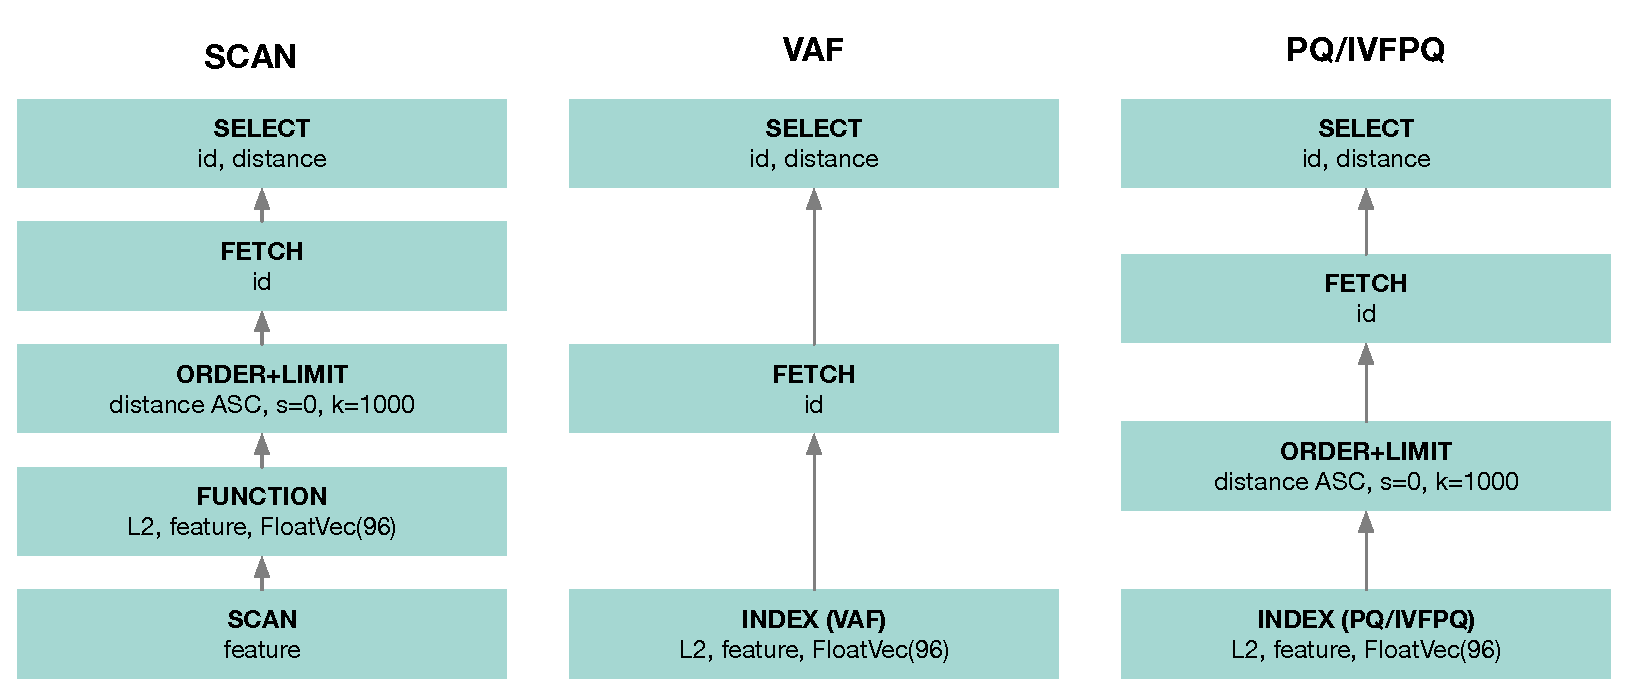
\includegraphics[width=\textwidth]{figures/bignns/cottontail/query-plan-nns}
        \caption{\acrshort{nns} and fetching of vectors.}
        \label{figure:cottontail_nns_fetch_plan}
    \end{subfigure}
    \hfill
    \centering
    \begin{subfigure}[b]{\textwidth}
        \centering
        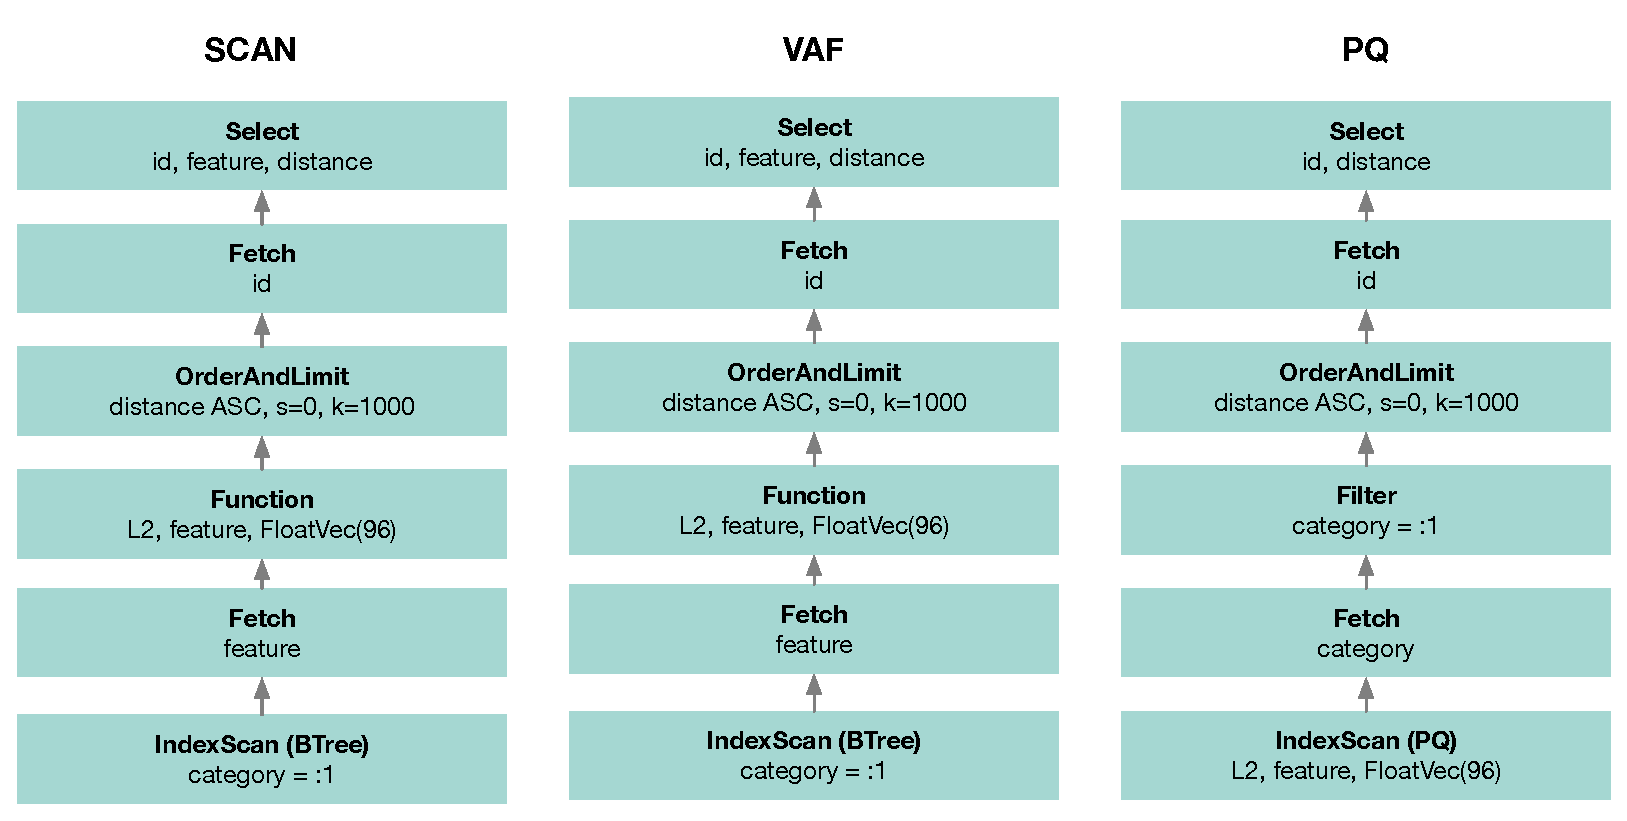
\includegraphics[width=\textwidth]{figures/bignns/cottontail/query-plan-hybrid}
        \caption{Hybrid query with Boolean filter.}
        \label{figure:cottontail_hybrid_plan}
    \end{subfigure}
    \caption{Execution plans produced by \cottontail{} for different query workloads prior to intra-query parallelisation. The use of the \acrshort{vaf} and \acrshort{pq} index was enforced using query hints.}
    \label{figure:cottontail_plans}
\end{figure}

Our second series of tests involved the combined \acrshort{nns} and fetching of the resulting vectors. One can see in \Cref{figure:cottontail_nns_fetch_plan} that in terms of execution plan, accessing this additional column does not make a difference. Since both the plan involving the entity scan and the \acrshort{vaf} index scan produce the \texttt{feature} column early on, there is not need to fetch it later. Only for the \acrshort{pq} index -- which uses a distance approximation that is obtained without accessing the \texttt{feature} column -- an additional fetch is needed, which again takes place after the order by and k-selection, to reduce IO. Consequently, the execution times are very similar to the simple \acrshort{nns} as one can see in \Cref{figure:cottontail_runtime} (NNS + Fetch). The numbers for a sequential scan range between $0.68 \pm 0.06 \, \si{\second}$ (5 million) and $10.53 \pm 0.29 \, \si{\second}$ (100 million). The impact of the additional fetching of $1000$ feature columns is negligible for the \acrshort{pq} index, which can be attributed to the fact that the fetch is pushed until after the $s,k$-selection. We expect the impact to become more important for larger values of $k$ but it should remain negligible since typically, $k << N$.

For the final measurement, we executed hybrid queries, i.e., \acrshort{nns} was restricted to a subset of the data that matches the predicate. The predicate involves a simple equality check that should effectively limit the exhaustive \acrshort{nns} to roughly $\frac{1}{10}$ of the collection. The values for a sequential scan range between $1.47 \pm 0.15 \, \si{\second}$ (5 million) and $25.6 \pm 0.39 \, \si{\second}$ (100 million) with very similar numbers for the \acrshort{vaf} and \acrshort{pq} indexes. To make sense of these values, we again turn to the query plans illustrated in \Cref{figure:cottontail_runtime} (Hybrid). The sequential scan took place with the help of a $B^{+}$-tree index, which speeds-up the Boolean filtering. Unfortunately, the current implementation of the \acrshort{vaf} index cannot natively accomodate Boolean predicates, since it constitutes a class 3 index replacement according to \Cref{definition:dfc_index_class_3} and therefore, a special implementation of the index would be required\footnote{It is, however, unclear if such an implementation would be beneficial in practice.}. Consequently, a $B^{+}$-tree was executed instead. In contrast, the \acrshort{pq} index can be combined with Boolead predicates, since it constitutes a class 1 index replacement according to \Cref{definition:dfc_index_class_1}. However, one can see in \Cref{figure:cottontail_runtime} (NNS + Fetch) that the advantage of using the is negligible.
This can be attributed to the fact that a fetch operation for the \texttt{category} column must be executed for every entry before executing the filtering. The IO overhead is much larger than the speed-up gained through the \acrshort{pq} index. This is confirmed by the numbers we see for the IVF\acrshort{pq} index, which restricts the scan to a small subset of the collection. Similarly to the IVF\acrshort{pq} index, the $B^{+}$-tree index does currently not allow for parallel evaluation due to \cottontail{}'s partitioning model. This is severly limiting for the hybrid queries and something that should be addressed in the future.

We refrain from visualising \acrshort{dcg} and recall values at this point due to space contraints but we can report that recall was always $1.0$ for sequential scan and \acrshort{vaf} and between $0.50$ and $0.30$ for \acrshort{pq} and IVF\acrshort{pq}, which can probably be attributed to a the small number of centroids that we used. The graphs showing these numbers can be found in \Cref{chapter:appendix_results}.

\subsection{Milvus}
For executing queries in Milvus, the mode of operation is a bit different than it is for \cottontail, since Milvus requires a data collection to be available in main memory, in order to be able to query it. Therefore, every query consists of two steps: Loading the collection and then executing the query once the collection is ready. We have obtained the ellapsed time for loading and query execution separately, so that we can reason about the individual components. The way queries can be specified is outlined in \Cref{listing:milvus_query}. We show the Python instead of the Java syntax, because it is less verbose and more readable, assuming, that the functionality of the two client libraries is identical.  

\begin{lstlisting}[language=Python, caption={Example of a similarity search query to Milvus in Python on a 2-dimensional vector with the prior loading of a data collection ``images''.}, label=listing:milvus_query, numbers=none]
    from pymilvus import Collection
    
    # Load an existing collection.
    collection = Collection("images")      
    collection.load()

    # Perform search.
    query = [[0.0, 0.0]]
    params = {"metric_type": "L2", "params": {"nprobe": 10}}
    results = collection.search(
        data=query, anns_field="feature", param=params, limit=10
    )
\end{lstlisting}

Accross all workloads, we compared the performance of two different types of indexes: The \texttt{FLAT} index is the equivalent of a sequential scan and it is the only index in Milvus that guarantees a recall of $1.0$. The \texttt{IVF\_SQ8} index uses an inverted file of clusters and limits search to a subset of these clusters based on the parameters provided by the user and an initial distance calculation between the query and the cluster centers. The approach is comparable to cluster pruning \cite{Chierichetti:2007Finding} or the two stage quantisation process described in \cite{Jegou:2010Product}, where each vector is mapped to an inverted list using a coarse quantiser. In addition to limiting the search space, the \texttt{IVF\_SQ8} index also compresses the \SI{4}{\byte} (\texttt{float}) into a \SI{1}{\byte} (\texttt{int8}) presentation, which significantly reduces memory and \acrshort{cpu} usage by up to 70\%. We built the \texttt{IVF\_SQ8} index beforehand using $4096$ clusters and instructed Milvus to search $1024$ and $2048$ clusters respectively.

In our first series of tests we executed the simple \acrshort{nns} workload. The results are depicted in Figure \Cref{figure:milvus_runtime} (NNS). We can summarise that even for brute-force search (\texttt{FLAT}), query execution speed is very impressive once a collection has been loaded into main memory. For our test collection, it took between $0.09 \pm 0.03 \, \si{\second}$ (5 million) and $1.3 \pm 0.18 \, \si{\second}$ (100 million) to execute a query, all the while retaining a perfect recall and \acrshort{dcg} of $1.0$. However, if one considers time to load a collection from disk to be part of the query time, these numbers rise to between $13.02 \pm 0.52 \, \si{\second}$ and $172.99 \pm 1.02 \, \si{\second}$. During that time, \cottontail{} can query the same collection $15$ (VAF) to $34$ (PQ) times while being able to switch between collections and using different indexes.

If one loads a collection once to then execute many queries thereafter, the performance provided by Milvus is very desirable as the cost of loading the collection can be amortised over time. However, if a large number of collections must be queried without the ability to predict which one, and not all collections can be pre-loaded, query exection time is expected to deteriorate. Furthermore, the requirement to load the collection prior to querying it turned out to be an insurmountable roadblock for the shard that contained 1 billion entries. Milvus was unable to load the collection as it ran out of available memory. We can confirm, that Milvus indeed used the entire \SI{376}{\giga\byte} available on the node.

In a attempt to aleviate the memory pressure, we also considered the \texttt{IVF\_SQ8} index, which seems a logical choice due to its data compression characteristics. Unfortunately, it did not resolve the problem of collection loading, since apparently, Milvus always loads all the available data. Nevertheless, there two interesting insights from the data:
\begin{enumerate*}[label=(\roman*)]
    \item \texttt{IVF\_SQ8} brings considerable speed-up for raw query execution time, especially for larger collections (roughly \SI{1}{\second} faster on 100 million shard),
    \item however, it exacerbates the performance impact of collection loading, since the necessary data structures must apparently be loaded in addition to the raw data.
\end{enumerate*} This confirms our suspicion, that Milvus indeed loads all data that belong to a collection, regardless of which one is being used.

The second series of tests involved the combined \acrshort{nns} and fetching of the resulting vectors. Unfortuntely, Milvus currently doesn't support the returning of vectors in a \acrshort{nns}, which is why this is a two-step process. First, the \acrshort{nns} is executed. Then the vectors for the resulting primary key's are fetched. We measure the time for both steps but do not reload the collection in between. The results are depicted in \Cref{figure:milvus_runtime} (NNS + Fetch). The additional fetching step, while cumbersome, does not seem to have a huge impact in cases where the \texttt{FLAT} index is used. However, use of the \texttt{IVF\_SQ8} index seems to lead to significant deterioration of the the query performance for the fetching step, adding approximately \SI{10}{\second} (5 million) to more than \SI{250}{\second} (100 million) to query execution time, even in cases where the query takes place in memory. We do not have an explanation for this and consider this to be abnormal behaviour.

Last but not least, we did execute hybrid queries, wherein \acrshort{nns} was restricted to a subset of the data that was filtered by a simple predicate. In Milvus this is a query primitive. The results are visualised in \Cref{figure:milvus_runtime} (Hybrid) and do not hold any surprises. In-memory query execution speed is again outstanding whereas time required to load a collection is significant. Interestingly, the \texttt{IVF\_SQ8}did not seem to have a negative impact on query execution speed.

\begin{landscape}
    \begin{figure}[p]
        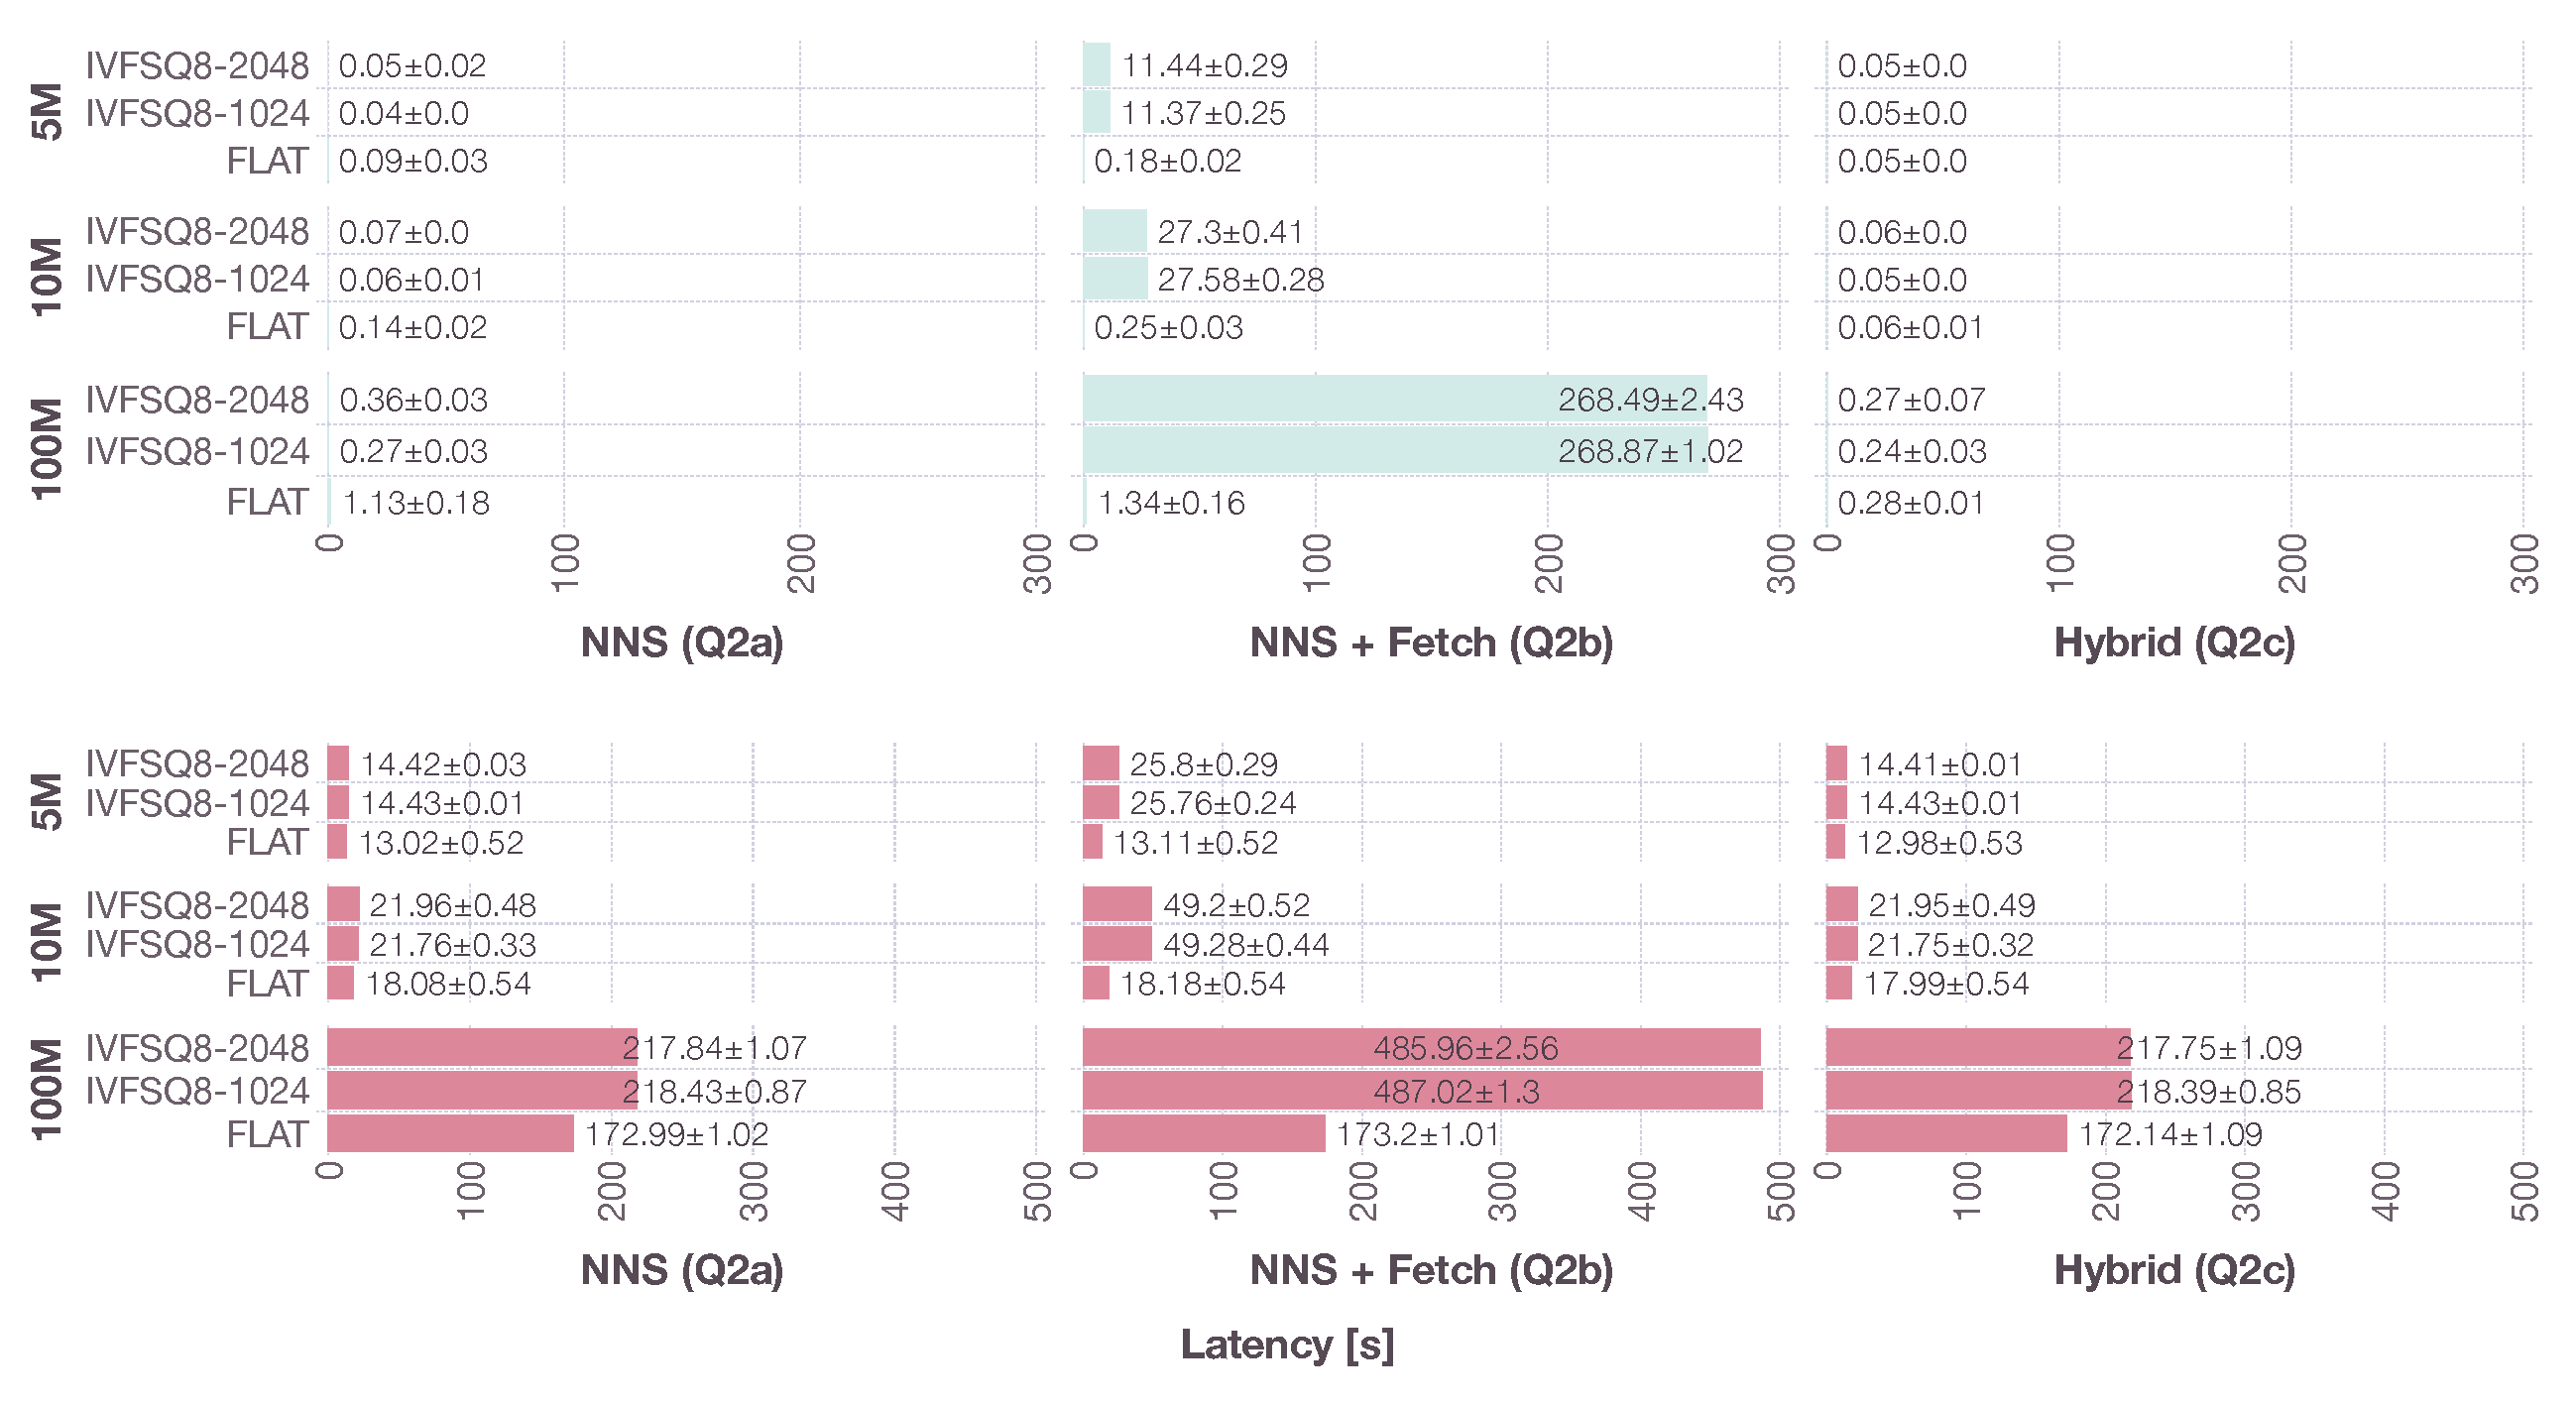
\includegraphics[width=1.6\textwidth]{figures/bignns/milvus/bignns-milvus}
        \caption{Milvus's latency in seconds for different workloads (x-axis) on different shards of the Deep 1B data set using different access methods (y-axis), with (red) and without (mint) time used for loading the data from disk.}
        \label{figure:milvus_runtime}
    \end{figure}
\end{landscape}

We again refrain from visualising \acrshort{dcg} and recall values but can report that recall was always $1.0$ for \texttt{FLAT} and around $0.99$ for all six queries using the \texttt{IVF\_SQ8} index.

\subsubsection{Qualitative Assesment}
While very convincing in terms of sheer execution speed, the current version of Milvus also has some limitations that we list here for future reference:

\begin{itemize}
    \item Milvus currently only supports the Euclidean and Inner Product distance for \acrshort{nns} on floating point embeddings.
    \item Milvus does not support proximity-based search strategies other than \acrshort{nns}. However, range search is due for the 2.2.0 release according to the official GitHub issue tracker.
    \item Milvus cannot retrieve the actual feature vectors as part of a \acrshort{nns}, i.e., they must be fetched in an additional query by looking them up based on the primary key. This issue is also due for being addressed in the 2.2.0 release.
    \item Milvus can only maintain a single index per feature column, effectively limiting the set of available distance functions to one, since most indexes must be trained for a specific index.
\end{itemize}

Furthermore, we have observed that as Milvus uses up all the memory during collection loading, it starts to behave rather eratic making it difficult to unload the collection again. In some of our runs, it even started to reload the same collection after a restart, effectively rendering the entire instance unusable for several hours.

\section{Adaptive Index Maintenance}
\label{section:evaluation_adaptive_index_maintenance}
\todo[inline]{Brute force vs. plain index vs. index with auxilary data structure}1